\section*{Цель}

Построение и исследование характеристик формирующих фильтров.

\section*{Порядок выполнения}

\begin{enumerate}
    \item Разработать программу для моделирования дискретного белого шума с интенсивностью $\sigma^2$, значение
    процесса в каждый момент времени должно подчиняться равномерному закону распределения.
    \item Разработать программу для моделирования дискретного белого шума с интенсивностью $\sigma^2$, значение
    процесса в каждый момент времени должно подчиняться нормальному закону распределения.
    \item Построить формирующий фильтр для моделирования экспоненциально коррелированного шума с
    параметрами $\Delta$ и $T$.
    \item Рассчитать спектральную плотность и установившиеся значения математического ожидания и дисперсии выхода
    формирующегося фильтра.
    \item Осуществить моделирование формирующего фильтра с начальными условиями, распределенными по закону $N(1,4)$,
    и входными сигналами из п.1 и п.2.
    \item На основе обработки экспериментальных данных оценить автокорреляционную функцию, установившиеся значения
    математического ожидания и дисперсии, законы распределения реализаций выхода формирующего фильтра.
\end{enumerate}

\section*{Исходные данные}

Заданные значения параметров $\sigma^2$, $\Delta$ и $T$ приведены ниже

\begin{align*}
    \sigma^2 & = 4 & \Delta & = 3 & T & = 50
\end{align*}

\newpage

\section*{Дискретный белый шум}

В первую очередь в настоящей лабораторной работе необходимо построить два генератора дискретного белого шума,
подчиняющегося равномерному и нормальному законам распределения соответственно.
Для каждого из генераторов далее приведены диаграммы значений выхода, а также графики функций распределения

\begin{figure}[h!]
    \centering
    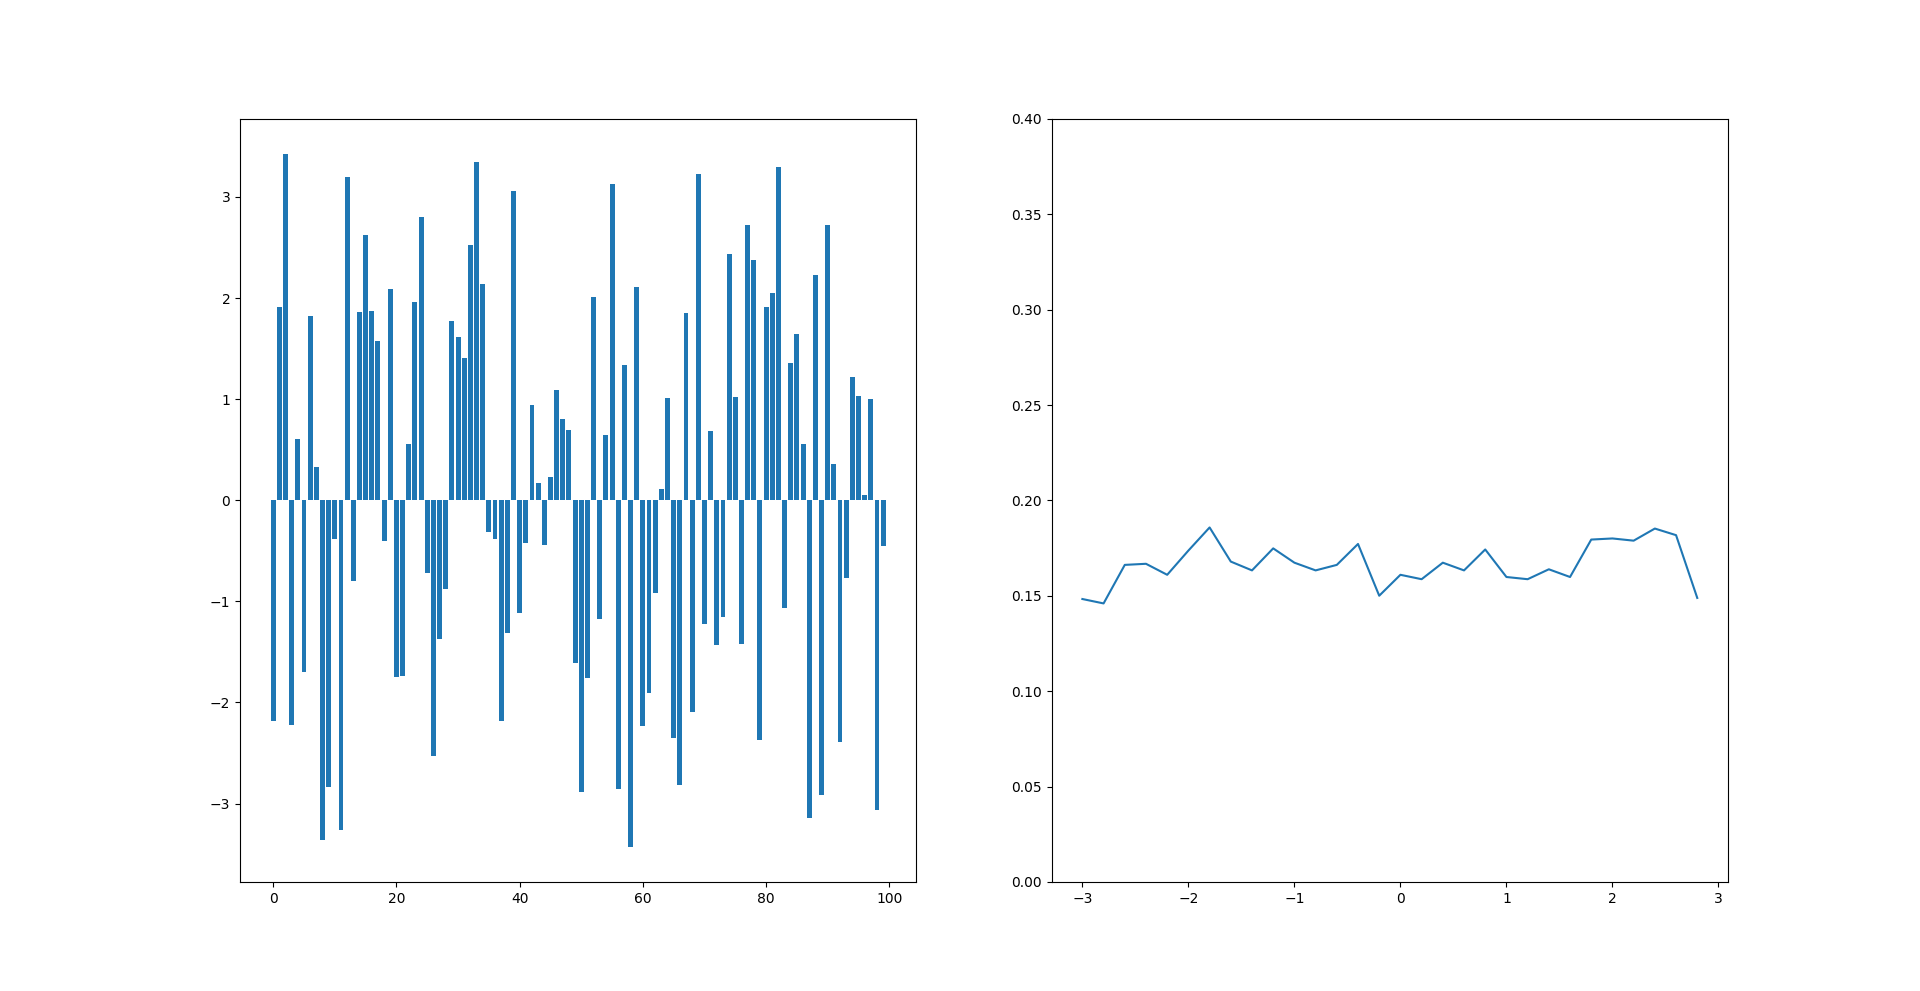
\includegraphics[width=0.8\textwidth]{\jobname/docs/img/uniform_noise.png}
    \caption{Диграмма значений выхода и график плотности вероятности равномерно распределенного дискретного белого шума}
\end{figure}

\begin{figure}[h!]
    \centering
    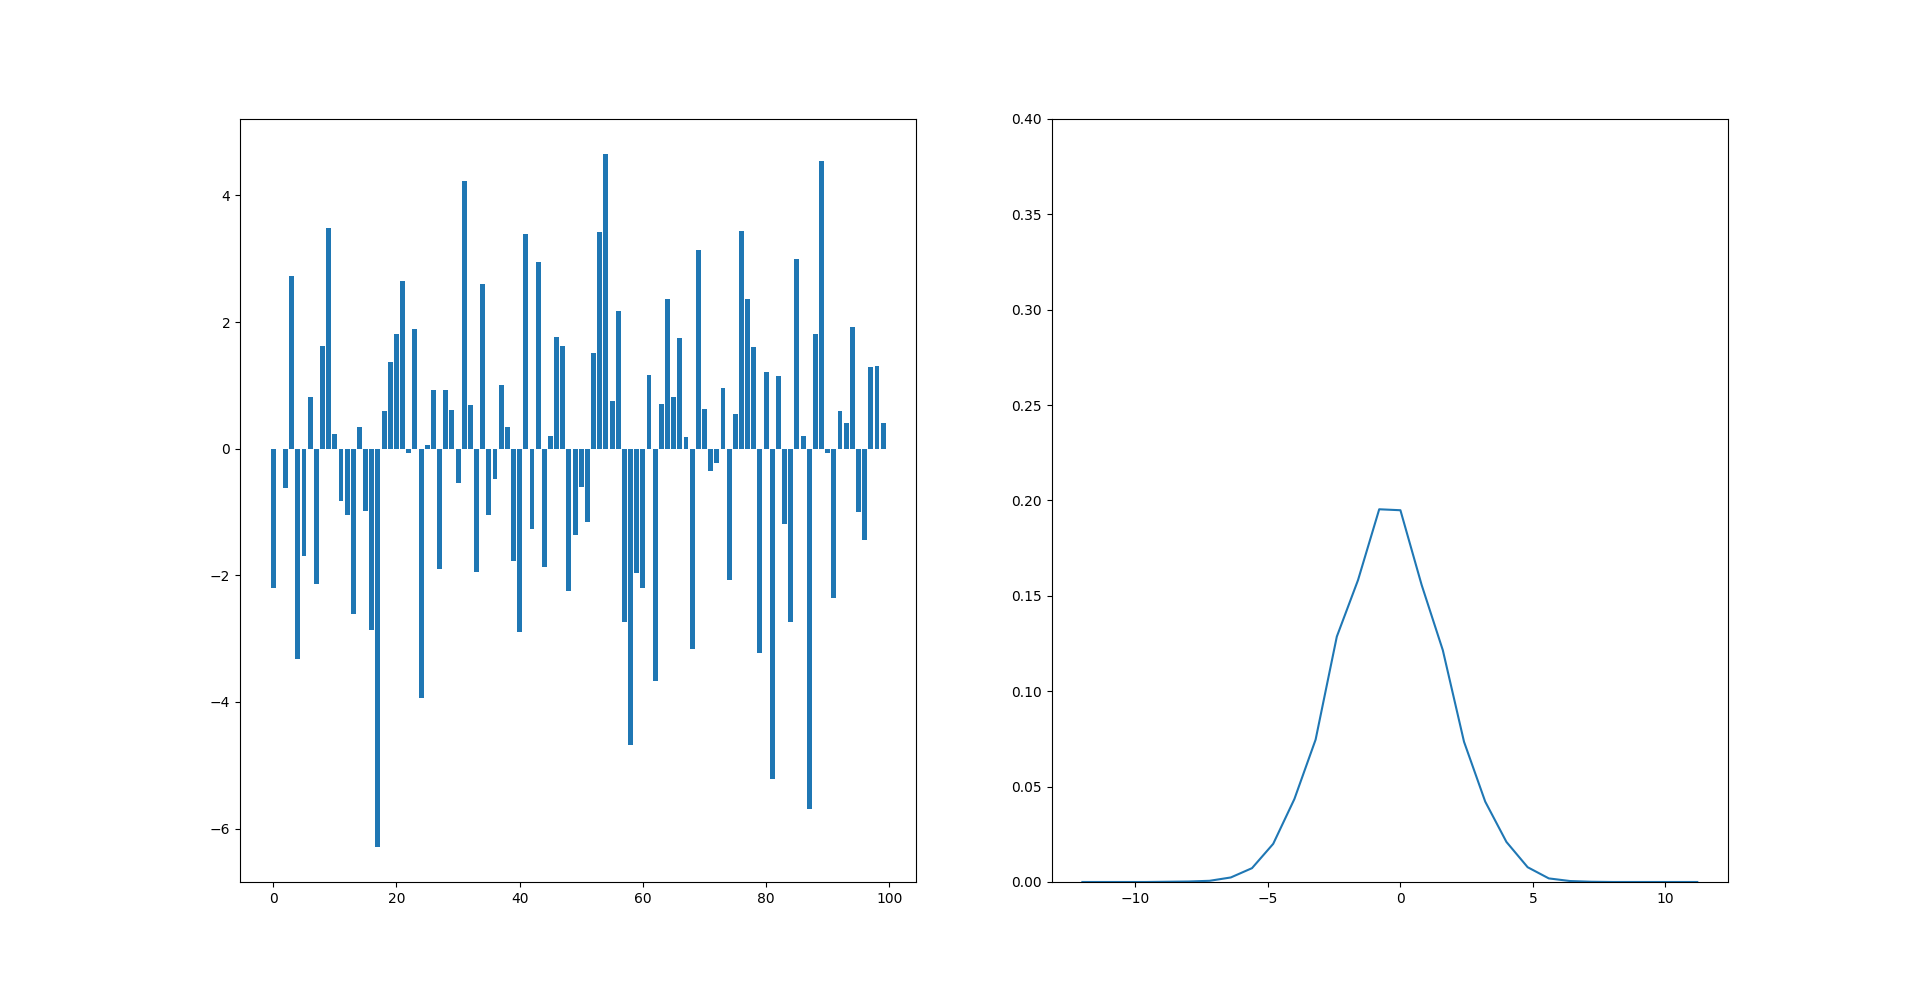
\includegraphics[width=0.8\textwidth]{\jobname/docs/img/normal_noise.png}
    \caption{Диграмма значений выхода и график плотности вероятности нормально распределенного дискретного белого шума}
\end{figure}

\clearpage

\section*{Формирующий фильтр}

Вторым шагом настоящей лабораторной работы следует создание формирующего фильтра для генерации экспоненциально
кореллированного белого шума.
Передаточная функция формирующего фильтра, а также полученное на ее основе уравнение вход-выход приведены ниже.

\begin{align*}
    H(z) & = \frac{\sqrt{1-\exp^{-2\frac{\Delta}{T}}}}{z-\exp^{-\frac{\Delta}{T}}}
\end{align*}

\begin{align*}
    y(k+1) & = -\exp^{-\frac{\Delta}{T}} y(k) + \sqrt{1-\exp^{-2\frac{\Delta}{T}}} v(k)
\end{align*}

Далее приведены графики автокорелляции и спектральной плотности выходов формирующих фильтров, построеных
с использованием двух видов вдохного распределения - равномерного и нормального.

\begin{figure}[h!]
    \centering
    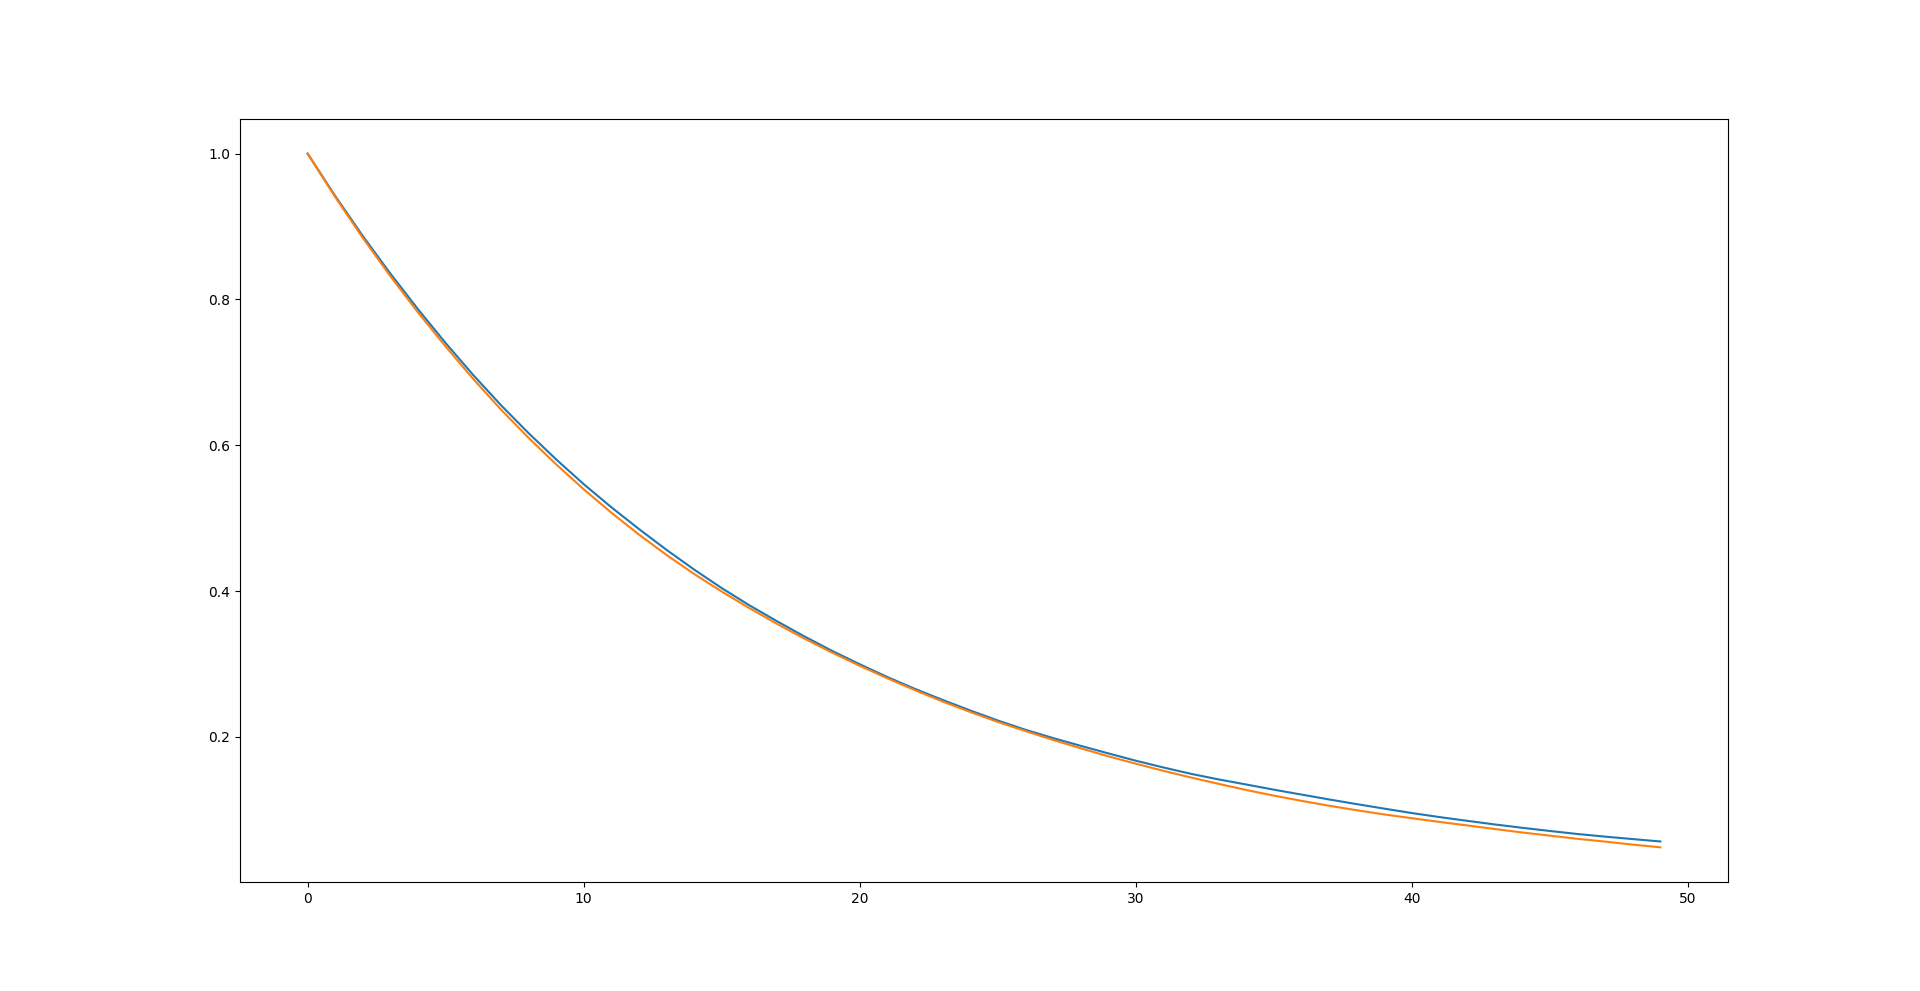
\includegraphics[width=\textwidth]{\jobname/docs/img/autocorellation.png}
    \caption{Графики автокорелляции выхода формирующих фильтров}
\end{figure}

\begin{figure}[h!]
    \centering
    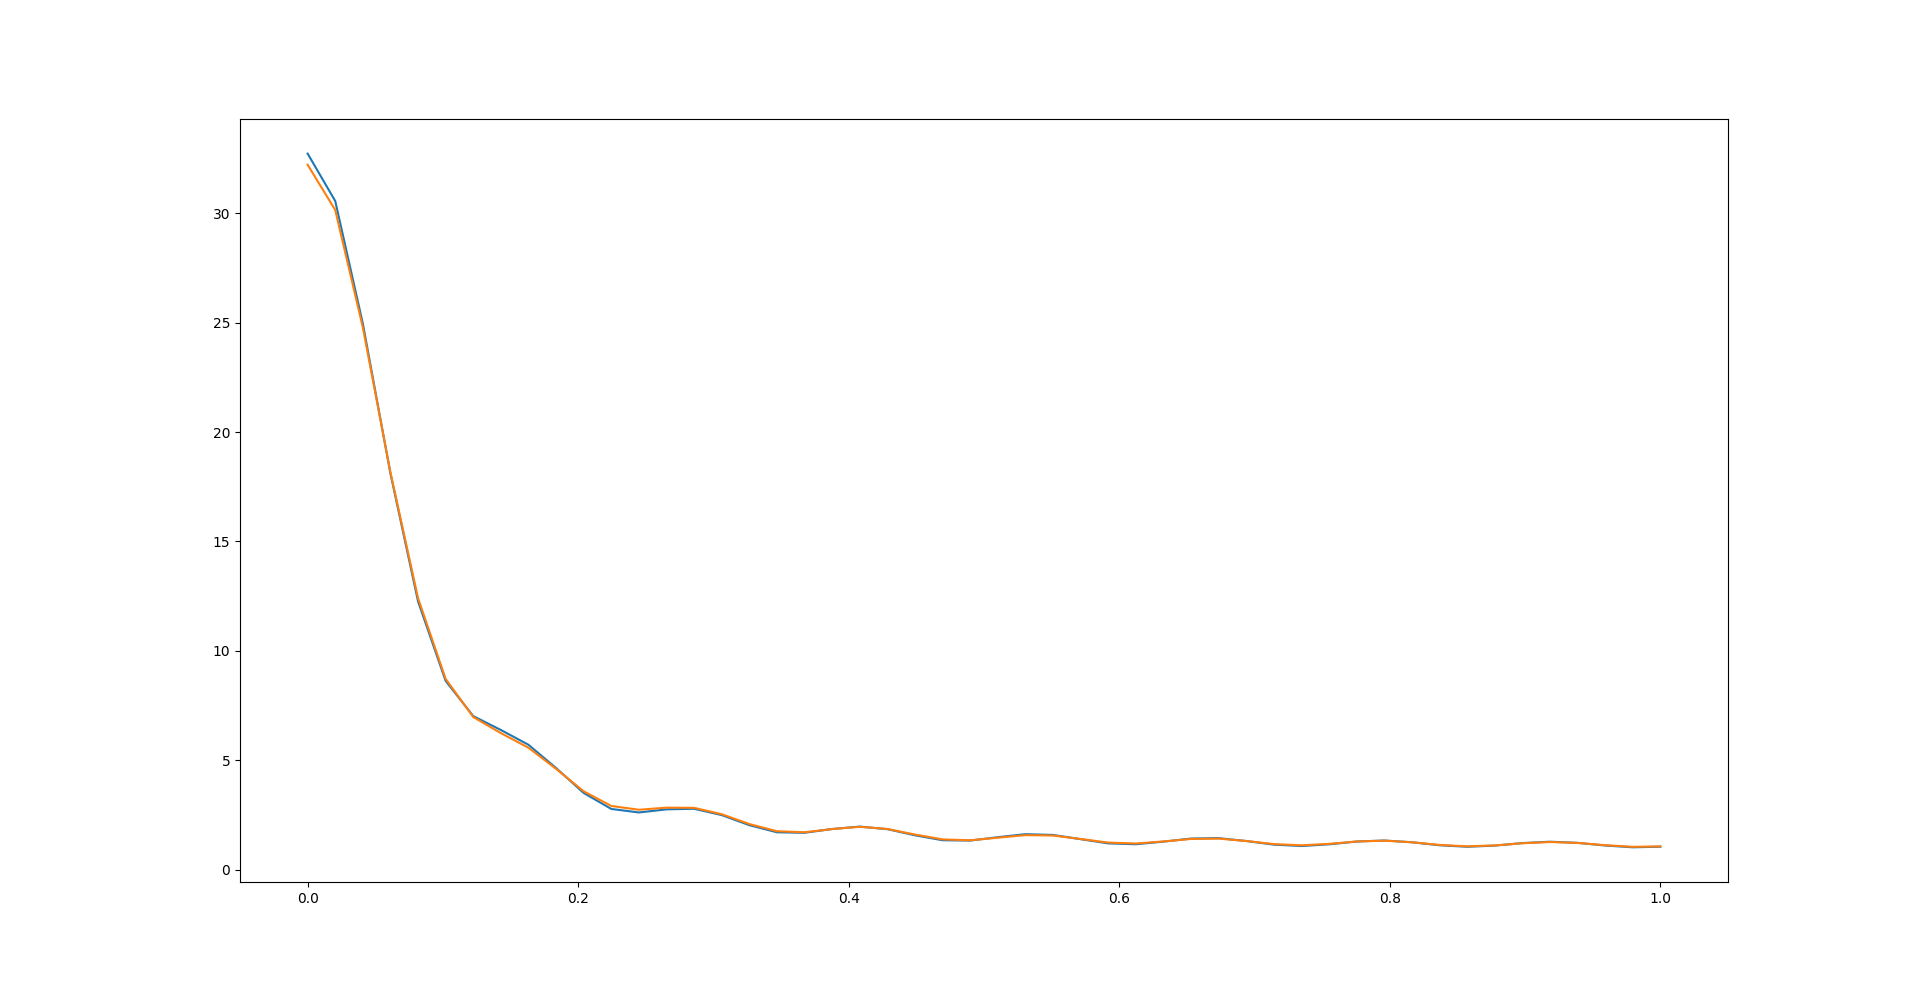
\includegraphics[width=\textwidth]{\jobname/docs/img/spectrum.png}
    \caption{Графики спектральной плотности выхода формирующих фильтров}
\end{figure}

Для каждого из двух входных распределений - равномерного и нормального - приведены диаграммы значений выхода,
а также графики плотности вероятности распределения.
Кроме того, указаны расчитанные установившиеся значения математического ожидания и дисперсии выхода формирующего
фильтра.

\clearpage

\subsection*{Равномерное распределение}

Установившиеся значения математического ожидания и дисперсии экспоненциально коррелированного белого шума,
построенного с использованием в качестве входного сигнала дискретного белого шума, подчиняющегося закону равномерного
распределения:

\begin{align*}
    M & = -0.007 & D & = 3.979
\end{align*}

Кроме того, на основе экспериментальных данных проверена гипотеза о нормальном законе распределения выхода формирующего
фильтра, соответствующие значения $Z$ и $\chi2$ приведены ниже.

\begin{align*}
    Z & = 169.245 & \chi2 & = 196.156
\end{align*}

Поскольку $Z < \chi2$, гипотеза о нормальном законе распределения принимается.

\begin{figure}[h!]
    \centering
    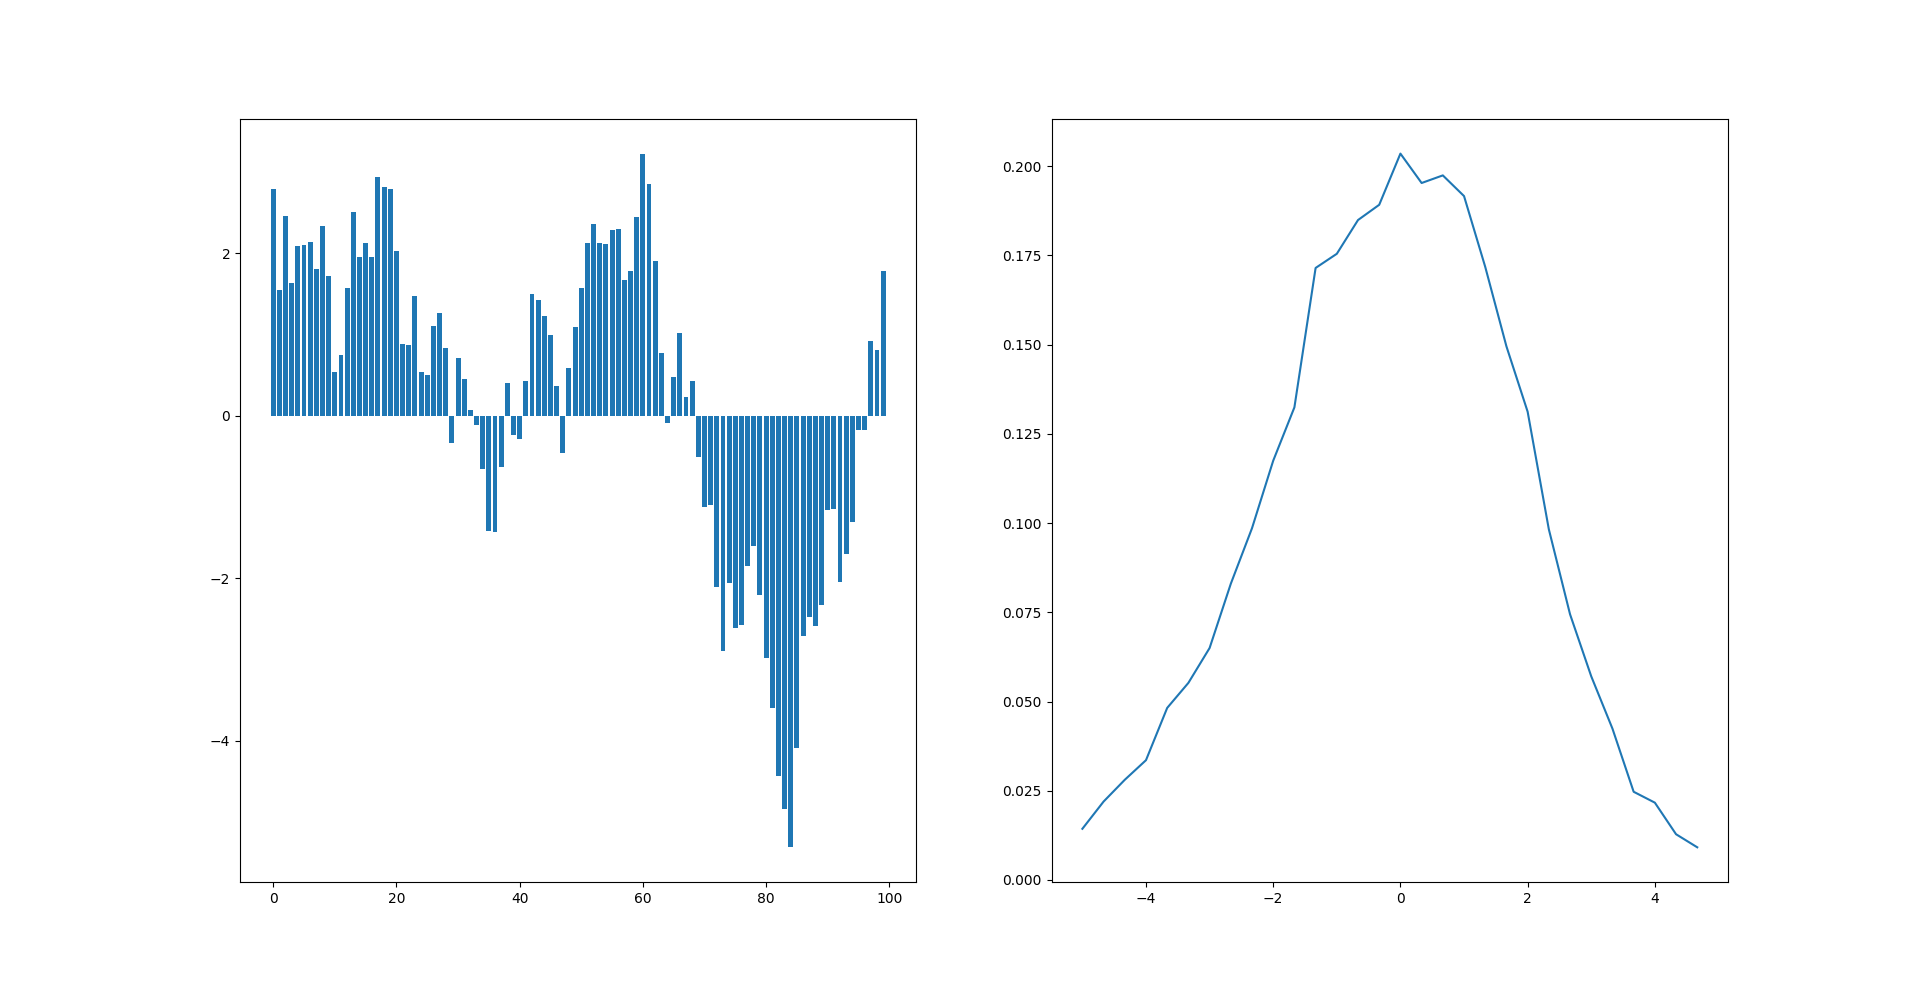
\includegraphics[width=\textwidth]{\jobname/docs/img/correlated_uniform_noise.png}
    \caption{Диграмма значений выхода и график плотности вероятности равномерно распределенного дискретного
    экспоненциально кореллированного белого шума}
\end{figure}

\clearpage

\subsection*{Нормальное распределение}

Установившиеся значения математического ожидания и дисперсии экспоненциально коррелированного белого шума,
построенного с использованием в качестве входного сигнала дискретного белого шума, подчиняющегося закону нормального
распределения:

\begin{align*}
    M & = 0.004 & D & = 4.014
\end{align*}

Кроме того, на основе экспериментальных данных проверена гипотеза о нормальном законе распределения выхода формирующего
фильтра, соответствующие значения $Z$ и $\chi2$ приведены ниже.

\begin{align*}
    Z & = 121.948 & \chi2 & = 196.156
\end{align*}

Поскольку $Z < \chi2$, гипотеза о нормальном законе распределения принимается.

\begin{figure}[h!]
    \centering
    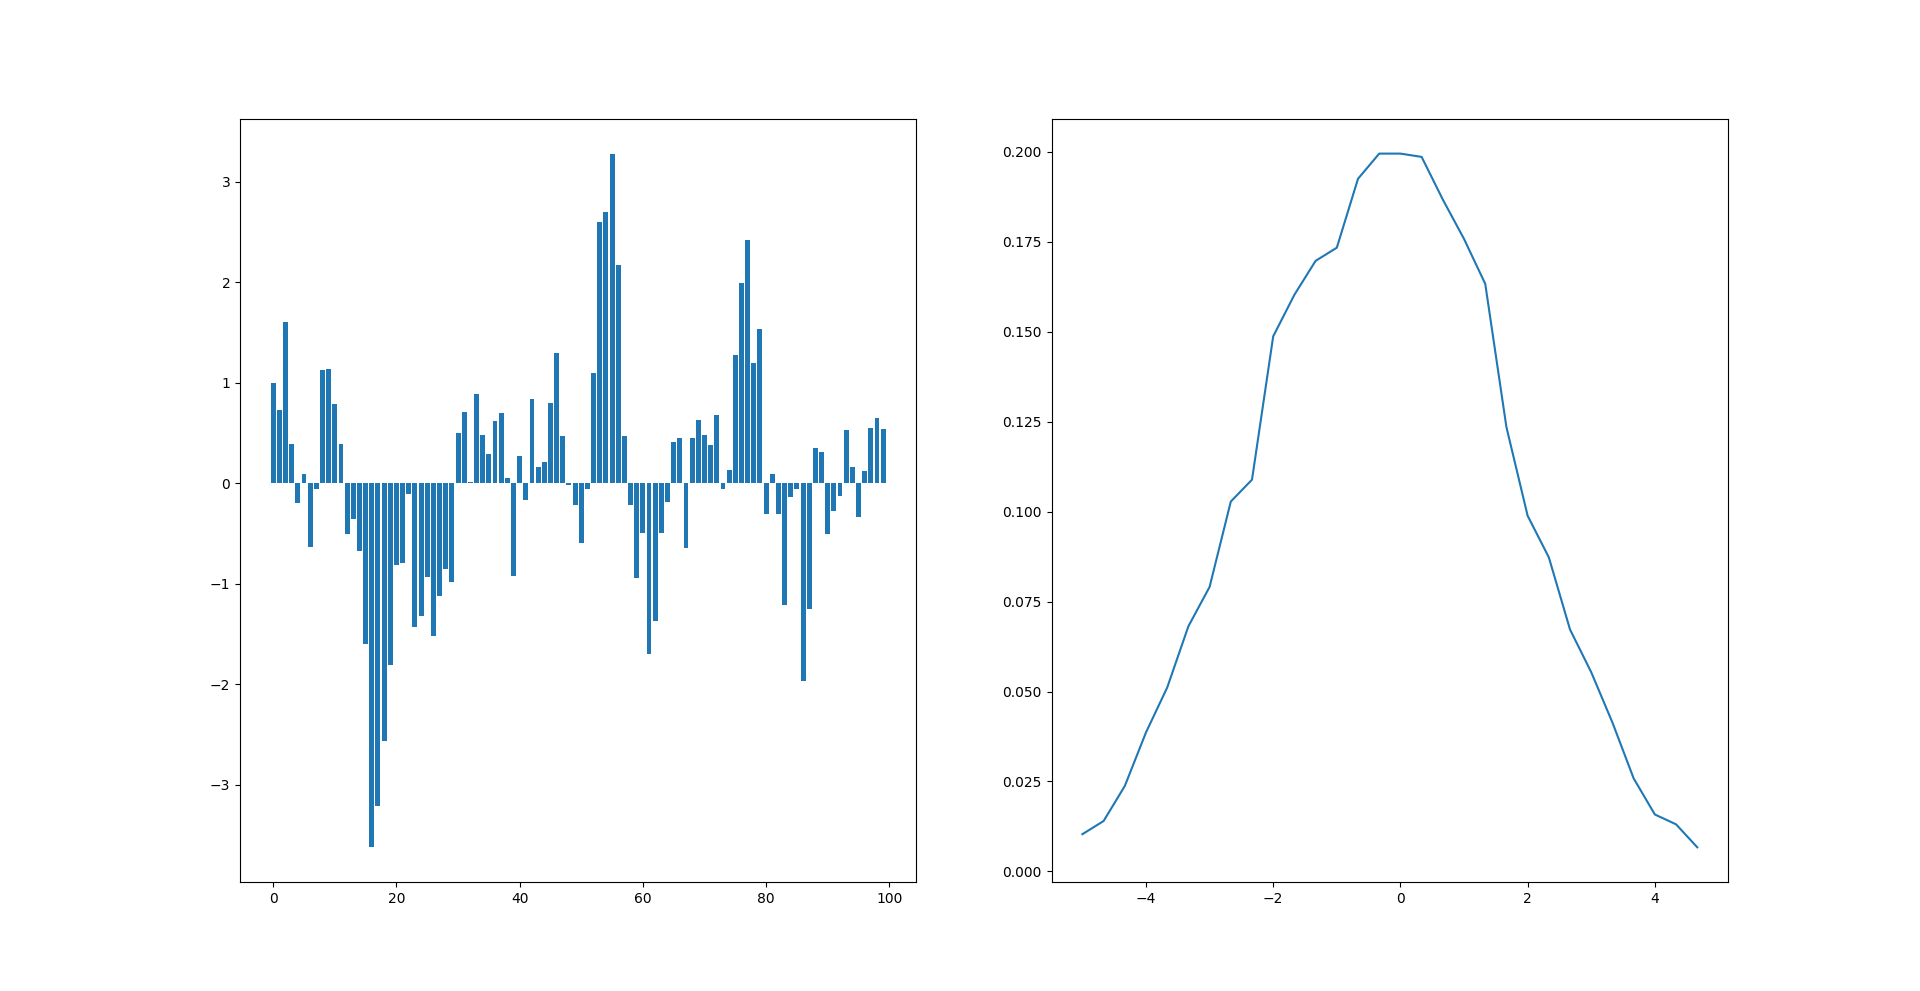
\includegraphics[width=\textwidth]{\jobname/docs/img/correlated_normal_noise.png}
    \caption{Диграмма значений выхода и график плотности вероятности нормально распределенного дискретного
    экспоненциально кореллированного белого шума}
\end{figure}

\clearpage

\section*{Выводы}

В ходе выполнения лабораторной работы были построены генераторы дискретного белого шума с различными законами
распределения - равномерным и нормальным.

На основе построенных генераторов была построена модель формирующего фильтра, позволяющего создать необходимый
уровень корреляции выходного сигнала на основе некоррелированного входного сигнала.

Разработанная модель использовалась для формирования экспоненциально кореллированного шума с различными видами
входного сигнала - равномерно и нормально распределенного.
Выходы построенных формирующих фильтров были исследован, в том числе были определены функция автокорреляции,
спектральная плотность, установившиеся значения математического ожидания и дисперсии выходного сигнала.

Кроме того были проверены гипотезы о законах распределения выхода формирующих фильтров. В обоих случаях, гипотеза
о нормальном законе распределениия подтвердилась.

\clearpage

\section*{Листинги}

\subsection*{Листинг основного скрипта}
\lstinputlisting[language=Python,texcl=true]{\jobname/lab.py}

\subsection*{Листинг скрипта, содержащего модель формирующего фильтра}
\lstinputlisting[language=Python,texcl=true]{\jobname/filter.py}

\subsection*{Листинг скрипта, содержащего генераторы}
\lstinputlisting[language=Python,texcl=true]{\jobname/../common/gen.py}

\subsection*{Листинг скрипта, содержащего утилиты}
\lstinputlisting[language=Python,texcl=true]{\jobname/../common/utils.py}

\subsection*{Листинг скрипта, инициализируещего логирование}
\lstinputlisting[language=Python,texcl=true]{\jobname/../common/log.py}
